%% main.tex
%% Copyright 2022 skyleaworlder
%
% This work may be distributed and/or modified under the
% conditions of the LaTeX Project Public License, either version 1.3
% of this license or (at your option) any later version.
% The latest version of this license is in
%   http://www.latex-project.org/lppl.txt
% and version 1.3 or later is part of all distributions of LaTeX
% version 2003/12/01 or later.
%
% This work has the LPPL maintenance status "maintained".
%
% This Current Maintainer of this work is skyleaworlder.
%
% This work consists of all the *.tex and *.sty files in
%   https://github.com/TJ-CSCCG/Tongji-Beamer
\documentclass{ctexbeamer}

\usepackage{amsthm}
\usepackage{biblatex}
\addbibresource{reference.bib}
\setbeamertemplate{bibliography item}[text]

\usetheme{tongji}

%Information to be included in the title page:
\title[LameCC - {https://github.com/leo4048111/LameCC}]{LameCC}
\subtitle{LameCC: 编译原理课程设计项目汇报}
\author[2050250 李其桐]{
    2050250 李其桐
}
\institute[CS Dept., CEIE, Tongji Univ.]{
    Computer Science and Technology Department, College of Electronic and Information Engineering(CEIE), Tongji University. \\
    同济大学\ 电子与信息工程学院\ 计算机科学与技术系\
}
\date{\today}

\begin{document}

\begin{frame}
    \titlepage
\end{frame}

%% introductioin.tex
%% Copyright 2022 skyleaworlder
%
% This work may be distributed and/or modified under the
% conditions of the LaTeX Project Public License, either version 1.3
% of this license or (at your option) any later version.
% The latest version of this license is in
%   http://www.latex-project.org/lppl.txt
% and version 1.3 or later is part of all distributions of LaTeX
% version 2003/12/01 or later.
%
% This work has the LPPL maintenance status "maintained".
%
% This Current Maintainer of this work is skyleaworlder.
%
% This work consists of all the *.tex and *.sty files in
%   https://github.com/TJ-CSCCG/Tongji-Beamer
\section{引言}
    \begin{frame}
    % “无序列表” 与 “有序列表” 使用
    \frametitle{引言}
        \footnotesize
        \begin{block}{项目提出背景}
            \begin{itemize}
                \item 	当前,ChatGPT已经发布并且对公众开放了服务接口,这无疑标志着一个人工智能的新纪元已然到来。通过ChatGPT的强势赋能,使得许多传统工作流都得到了极大的颠覆与创新,在达到更高效率的同时也能够确保质量。本项目正是在这一背景下,基于ChatGPT的公开API接口,搭建一个能够根据用户的自然语言描述需求,自动生成Markdown格式文档,然后通过Markdown解析器处理文件文本内容从而生成ppt的软件系统,从而能够在人们的实际文档设计与编写工作中,以一个可靠软件助手的姿态提供辅助,有效提升人们的工作效率。
            \end{itemize}
        \end{block}

        \begin{block}{项目意义}
            \begin{enumerate}
                \item 为响应在互联网传统工作方式中,企业内部、学生和个人对PPT文档的自动化生成和在线编辑需求而进行设计和开发。
                \item 为用户节省编辑成本,提升编辑效率,拥有广泛的应用前景。
                \item 对于其它竞品的相关功能特性进行研究分析,并且在其基础上进行精炼、完善,同时围绕核心业务设计并且实现额外的使用子功能模块。
            \end{enumerate}
        \end{block}
    \end{frame}


\section{项目详细设计}
\begin{frame}
    \frametitle{类设计}
    \footnotesize
    \begin{itemize}
        \item {File类:用于储存读入的源文件内容,提供了操作文件的相关接口,包括数据获取、移动行号、信息记录等等}
        \item {Lexer类:词法分析器实现主体类,在一遍过程中为语法分析器提供nextToken()接口用于推进分析过程}
        \item {Parser和LR1Parser类:实现了递归下降和LR1分析两种语法分析方法的语法分析器实现主体类,输出相同的AST数据结构}
        \item {LLVMIRGenerator和IRGenerator类:分别使用语法制导翻译技术,输出LLVM IR和四元式形式表示的中间代码序列}
        \item {CodeGenerator类:使用LLVM IR中间代码序列作为输入,执行代码优化逻辑后输出可执行的目标文件}
        \item {相关工具类:包括错误处理、日志记录、运行时参数解析等于项目实现相关的工具类,可在源码中查看,此处不再赘述}
        \item {AST节点类:本实验中的AST节点类设计参考了Clang源码中的设计架构,为每种实现需求中的文法符号实现了对应的节点类型定义,此处重点阐述其中所有类型的具体含义}
    \end{itemize}
\end{frame}

\section{项目功能扩充}
\begin{frame}
    \frametitle{增加单词的数量}
    \footnotesize
    {编译器支持的所有关键字在TokenType.inc中定义,可进入源码查看}
\end{frame}

\begin{frame}
    \frametitle{将整常数扩充为实常数}
    \footnotesize
    {本次项目开发中实现的词法分析器已经能够支持按照C语言语法标准读入实常数,包括整形数和浮点数。此处给出所有接受的浮点表示形式如下:}
    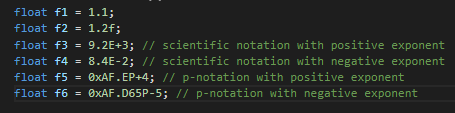
\includegraphics[width=\textwidth]{contents/figure/float.png}
\end{frame}

\begin{frame}
    \frametitle{增强编译器的编译能力}
    \footnotesize
    {编译器在基础项目开发要求的基础上扩展了编译能力,支持包括数组、指针、GCC风格内联汇编语句等等一系列基本C语言语法规范,具体支持的所有C语言语句可以到源码下的test.c测试源码文件中查看}
\end{frame}

\begin{frame}
    \frametitle{较为完善的错误处理}
    \footnotesize
    {对于输入的源码文件,编译器能够给出存在词法错误的token(包括错误类型和位置)还有存在语法错误的语句(包括错误类型和位置),便于开发人员定位错误并且修改}
\end{frame}

\begin{frame}
    \frametitle{从词法分析到可执行文件生成的全套解决方案}
    \footnotesize
    {本编译器最终生成的目标代码文件(例如x86-64汇编或者x86汇编),可以直接输入到对应的第三方编译环境中(例如GCC,Clang等),进一步通过第三方编译环境提供的链接器与第三方实现的标准类库进行链接,最终生成能够在对应平台上正确执行的可执行文件,从而更加直观地查看编译器对于源码逻辑编译的正确性}
\end{frame}
%% summary.tex
%% Copyright 2022 skyleaworlder
%
% This work may be distributed and/or modified under the
% conditions of the LaTeX Project Public License, either version 1.3
% of this license or (at your option) any later version.
% The latest version of this license is in
%   http://www.latex-project.org/lppl.txt
% and version 1.3 or later is part of all distributions of LaTeX
% version 2003/12/01 or later.
%
% This work has the LPPL maintenance status "maintained".
%
% This Current Maintainer of this work is skyleaworlder.
%
% This work consists of all the *.tex and *.sty files in
%   https://github.com/TJ-CSCCG/Tongji-Beamer
\section{总结}
    \begin{frame}{总结}
        “永夜星弓” 系统已在我校试运行 2 个月。试运行期间,上报内卷行为 300'000 起,成功制止 280'000 次轻微内卷行为、10'000 次中等内卷行为以及 10'000 次重度内卷行为。

        \begin{center}
            感谢在毕业设计实现过程中提供指导的老师们!

            感谢在这百余天中一直陪伴我的家人和同学们!

            感谢这个美丽的世界给了我从大学毕业的机会!
        \end{center}

        \begin{center}
            谢谢各位!请多多指教!
        \end{center}
    \end{frame}

\end{document}
